\documentclass[10pt]{beamer}
\usetheme{metropolis}           % Use metropolis theme
\usepackage[utf8]{inputenc}
\usepackage{amsmath,amsfonts,amssymb}
\usepackage{dsfont}
\usepackage{graphicx}
\usepackage{caption}
\usefonttheme[onlymath]{serif}


\def\R{\mathbb R}

\def\T{\mathbb T}

\title{Calcul paradifférentiel et théorème d'Arnold}
\date{14 Mai 2024}
\author{Sacha Ben-Arous, Mathis Bordet}
\institute{ENS Paris-Saclay}
\begin{document}
  \maketitle
\begin{frame}
\tableofcontents
\end{frame}  

\section{Calcul paradifférentiel}


\begin{frame}{Multiplicateurs de Fourier}
\begin{figure}
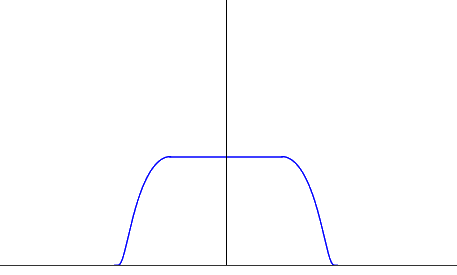
\includegraphics[width=0.35\textwidth]{psi.png}
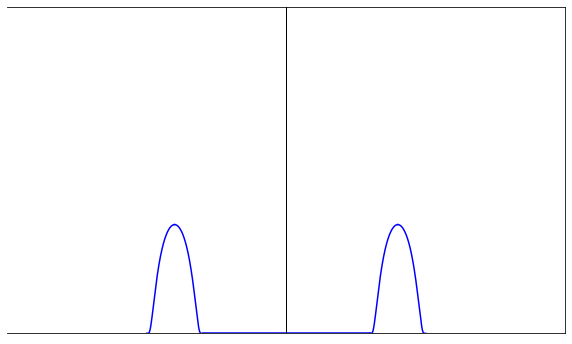
\includegraphics[width=0.35\textwidth]{chi.png}
\end{figure}
On définit les opérateurs de la décomposition de Littlewood-Paley de la manière suivante :
\[
\text{Pour } u \in \mathcal{S}', \quad \widehat{\Delta_{-1} u} := \psi \cdot \hat{u}, \quad \widehat{\Delta_{k} u} := \chi(2^{-k} \cdot) \cdot \hat{u} \ \text{ si } k \geq 0
\]
\[ S_n u := \sum_{k=-1}^{n-1} \Delta_k u \]
On a que :
\[ \lim_{n \to \infty} S_n u = u \]
\end{frame}


\begin{frame}{Décomposition régularisante}
\begin{itemize}
\item Régularisation: si $u\in L^2$, alors pour tout $n\in \mathbb{N}, S_n \in \mathcal{S}$.
\item[•] Presque comme une base hilbertienne : pour tout $u\in L^2(\mathbb{R}^d)$, 
\[\sum_{k \geq -1} \|\Delta_k u \|^2_{L^2} \leq \| u \|^2_{L^2} \leq 2 \sum_{k \geq -1} \|\Delta_k u \|^2_{L^2}. \]
\end{itemize}
\end{frame}


\begin{frame}{Caractérisations d'espaces fonctionnels}
 Pour $s\in \mathbb{R}^+$, $u\in L^2(\mathbb{R}^d)$, on a : \[ u\in H^s(\mathbb{R}^d) \Leftrightarrow \sum_{k\geq -1}2^{2ps}\|\Delta_k u \|_{L^2}^2 < +\infty. \] 
 Pour $r\in \mathbb{R}^+ \setminus \mathbb{N}$, $u\in L^\infty(\mathbb{R}^d)$, on a : \[ u\in C^r(\mathbb{R}^d) \Leftrightarrow \sup_{k \geq -1} 2^{k\alpha}\|\Delta_ku\|_{L^\infty} < +\infty . \] 
\end{frame}


\begin{frame}{Paraproduits}
\begin{align*}
uv &=\sum_{k=-1}^{+\infty}\Delta_kuS_{k-2}v  \ +  \sum_{k=-1}^{+\infty}\Delta_kvS_{k-2}u \ + \sum_{|k-j|\leq 2} \Delta_ku\Delta_ju \\
&= T_vu + T_uv + R(u,v)
\end{align*}

\begin{itemize}
\item[•] $\forall s\in \R^+, u \in L^\infty, v\in H^s,$
\[ \|T_uv\|_{H^s} \leq C_s \|u\|_{L^\infty} \|v\|_{H^s} \]
\item[•] $\forall \alpha \in \R^+, u \in L^\infty, v\in C^\alpha_*,$
\[\|T_uv\|_{C^\alpha_*} \leq C_\alpha \|u\|_{L^\infty} \|v\|_{C^\alpha}\]
\end{itemize}
\end{frame}

\begin{frame}{Paralinéarisation}
\begin{itemize}
\item[•]Soit $F$ une fonction $C^{\infty}$ de $\R$ telle que $F(0)=0$. Si $u\in H^s(\R^d)$, avec $\rho := s - \frac{d}{2}>0 $, alors 
\[F(u) - T_{F'(u)}u \in H^{s+\rho}(\R^d).\]
\item[•]
Soit $s,r>0$, et $a,b\in C^r_*(\T^d)$. Alors 
\[R_{CM}(a,b) := T_a \circ T_b - T_{ab} \]
est un opérateur continu de $H^s(\T^d)$ dans $H^{s+r}(\T^d)$
\end{itemize}
\end{frame}



\section{Difféomorphismes du cercle}
\begin{frame}{Dynamique en dimension 1}
    On considère le cercle $\mathbb{S}^1 := \left\{z, |z|=1 \right\}$, ainsi que le plongement $\Pi : \mathbb{R} \mapsto \mathbb{S}^1, t \mapsto e^{2i\pi t}$. \\
    
Pour $f:\mathbb{S}^1 \mapsto \mathbb{S}^1$, on dit que $F: \mathbb{R} \mapsto \mathbb{R}$ est un relèvement si $\Pi \circ F = f \circ \Pi$, i.e $f(e^{2i\pi t}) = e^{2i\pi F(t)}$

\textbf{Lemme :} Si $f$ est un $\mathcal{C}^k$-difféomorphisme du cercle, alors il existe un relèvement de $f$ qui est un $\mathcal{C}^k$-difféomorphisme (de $\mathbb{R}$). \\~\\

Dans la suite, on considèrera a minima des homéomorphismes, ainsi que leur relèvements réguliers associés.
\end{frame}

\begin{frame}{Nombre de rotation et Théorème Poincaré }
    Si $f$ est un homéomorphisme, $F$ un relèvement, et $x\in \mathbb{R}$, la suite $\displaystyle (\frac{F^n(x)}{n})_{n\in \mathbb{N}}$ converge vers une limite indépendante de $x$, notée $\rho(F)$. On définit alors $\rho(f):= \rho(F) \mod 1$. \\~\\
   
\textbf{Théorème (Poincaré) :} Si $f$ est un homéomorphisme de nombre de rotation $\alpha$ irrationnel, alors $f$ est semi-conjugué à $R_\alpha$, i.e il existe $h$ continue telle que $h \circ f = R_\alpha \circ h$. \\~\\
\end{frame}

\section{Théorème d'Arnold}
\begin{frame}
\frametitle{But}
Le But du théorème d'Arnold est déterminé la régularité des conjugaison d'un homéomorphisme g d'angle de rotation $\alpha$ irrationnelle proche de la rotation $R_\alpha$. c'est a dire résoudre :
$$\eta(x + \alpha)= g \cdot \eta(x)$$
\\
d'inconnue $\eta$.
\end{frame}
\begin{frame}
\frametitle{Cadre}
On écrit alors :
\[ g(x) = R_\alpha + f(x) \]
avec $f$ "assez petit". \\
On cherche alors $\eta= id + u $. 
L'équation a résoudre:
$$\eta(x + \alpha)= g \cdot \eta(x)$$
devient alors : 
$$ \Delta_\alpha u= f \cdot (id +u)  \; \text{avec  } \Delta_\alpha u(x)= u(x+\alpha) - u(x)$$

\end{frame}

\begin{frame}
\frametitle{Perte de régularité}
En voulant résoudre
$$ \Delta_\alpha u = h (x) $$
On a que 
\[ (\exp(2 i \pi n \alpha)-1)\widehat{u} (n) = \widehat{h} (n) \]
Avec la condition diophantienne:
$$ \|\frac{q \alpha}{\pi}-p|\geq \frac{1}{\gamma q^\sigma}$$
cela induit la perte de régularité suivante, si $h \in H^{s+\sigma}$ alors $\Delta_\alpha^{-1}h \in H^{s}$


\end{frame}


\begin{frame}
\frametitle{Enoncé et Preuve}
L'idée de la preuve est de transformer l'équation  :
$$ \Delta_\alpha u= f \cdot (id +u)$$
en une equation de la forme:
$$u = \Delta_\alpha^{-1} Lu$$
De telle sorte que $L$ compense les pertes de $\Delta_\alpha^{-1}$ grace au théorème de paralinéarisation.
\\
On en conclut que pour que la conjugaison soit dans $H^s$, il faut que $f$ soit dans $H^{s+\sigma + \varepsilon}\cap C^{N_s+1}$
\end{frame}


\begin{frame}
\section{Conclusion}
\end{frame}

\end{document}

